\documentclass[10pt, twocolumn]{article}

%math
\usepackage{amsmath}
\usepackage{amssymb}
\usepackage{mathtools}
%logic
\usepackage{pgffor}
\usepackage{ifthen}
%science
\usepackage{siunitx}
\usepackage[version=4]{mhchem}
%language
\usepackage[english]{babel}
%formatting
\usepackage[a4paper, portrait, margin=1in]{geometry}
\usepackage{cuted}
\usepackage[small]{titlesec}
\usepackage[hidelinks]{hyperref}
\usepackage{parskip}
%images and plots
\usepackage{graphicx}
\usepackage[justification=centering]{caption}
\usepackage{subcaption}
\usepackage{float}
\usepackage{pgf}
\usepackage{import}
%tables
\usepackage{booktabs}
\usepackage{makecell}
%citation, quatation and lists
\usepackage[style=numeric,maxcitenames=2,sorting=none,doi=false,
url=false,isbn=false,eprint=false]{biblatex}
\usepackage[noabbrev,nameinlink]{cleveref}
\usepackage{csquotes}
\usepackage[nottoc]{tocbibind}
\usepackage{acro}


%setup plugins
\addbibresource{literature.bib}
\crefformat{equation}{#2(#1)#3}
\captionsetup{justification=centering}
\hypersetup{colorlinks=true,linkcolor=blue}


\DeclareSIUnit\angstrom{\text {Å}}
\DeclareSIUnit\bar{bar}
\sisetup{
	range-phrase = { to }
}

% Custom \citeauthoryear command with hyperref -> Rost et al. (2019) 
\DeclareCiteCommand{\citeauthoryear}
{\boolfalse{citetracker}%
\boolfalse{pagetracker}%
\usebibmacro{prenote}}
{\ifciteindex
{\indexnames{labelname}\indexfield{year}}
{}%
\printtext[bibhyperref]{%
    \printnames{labelname}%
    \setunit{\addspace}%
    \printtext{(}%
    \printfield{year}%
    \printtext{)}}}
{\multicitedelim}
{\usebibmacro{postnote}}

%  setup custom commands
\newcommand{\imcite}[2][]{From \cite[#1]{#2}.}
\newcommand{\imcitetwo}[2][]{Based on \cite[#1]{#2}.}
\newcommand{\integral}[4]{\int_{#1}^{#2} #3 \mathrm{d} #4}
\newcommand{\derivative}[2]{\frac{\mathrm{d}}{\mathrm{d} #1} #2}

%set up acronyms
\DeclareAcronym{pld}{
	short=PLD,
	long=pulsed laser deposition
}

\DeclareAcronym{pvd}{
	short=PVD,
	long=physical vapor deposition
}

\DeclareAcronym{mbe}{
	short=MBE,
	long=molecular beam epitaxy
}

% Document
\begin{document}
\pagenumbering{arabic}
\begin{strip}
	\begin{centering}
	\huge Semiconductor Physics Laboratory \RN{1}\\
	\LARGE A2: Scanning electron microscopy \\
	\vspace{0.35cm}
	\normalsize Simon Legtenborg, 3773994 \\ 
	\normalsize Experiment conducted on 22.11.2024 \\
	\vspace{1cm}
\end{centering}

\end{strip}
Die Breite einer Spalte beträgt: \the\columnwidth
%\paragraph{Abstract}
This lab report explores various applications of a scanning electron
microscope.
Using secondary electron detection, the topography of an unknown
semiconductor sample is analyzed.
Additionally, material characteristics are determined through
X-ray emission and backscattered electrons.

\section{Pulsed Laser Deposition}
The investigation of thin films is essential in science and 
technology and has led to countless inventions such as integrated circuits, 
microchips and many more. 
Therefore, it is crucial to have a reliable and precise way to fabricate thin films. 
One method, which is not only reliable, but also flexible and comparatively inexpensive,
is \ac{pld}. 
Therefore, this protocol aims to present the \ac{pld} structure and its working
principles.

\subsection{The PLD Process explained in steps}
In \ac{pld}, the process begins with a bulk material that will form the thin film.
This material source, called target, is installed into a vacuum chamber along with a 
substrate that serves as the foundation and growth template of the film.
For this lab course, a \ce{ZnO} target and a c-sapphire substrate was used.
A high-power pulsed laser in the ultraviolet spectral range is focused through a lens 
and directed through a window into the vacuum chamber, where it hits the target. 
During every laser pulse, the target material begins to ablate and vaporizes. 
The vaporized material interacts with the laser photons as well and thus excites into a 
plasma. 
This plasma is directed towards the substrate, where it condenses.
After each pulse, some material is added and after a fixed number of pulses,
a thin film is deposited on the substrate. 

The laser-target interaction is a complex and nonequilibrium process and therefore
hard to model analytically.
Laser photons are absorbed by the target material and excite the electronic system.
Due to the electron phonon interaction, this electronic excitation is converted 
into thermal, chemical and mechanical energy and leads to the ablation and evaporation
of the material.
The ejected species expand into the vacuum, interact with the laser and form a plasma
plume. 
This plume consists of electrons, atoms, ions, molecules and clusters and is directed 
towards the substrate.

\Ac{pld} runs inside a vacuum chamber under ultrahigh vacuum or under a controlled 
background gas pressure.
The background gas can be chosen, oxygen, nitrogen or argon are common candidates.
The substrate is normally heated using a resistive or laser heater.

\Ac{pld} is very flexible for investigating thin film materials.
It is applicable for a large material library, including oxides, nitrides and even
metals. 
For most materials it also ensures stoichiometric transfer from the target to the film,
but this is not guaranteed.

\subsection{Design of a \ac{pld} System}
In this section the structure of a \ac{pld} system shall be discussed.
\ac{pld} is a \ac{pvd} technique and thus characterized by a process in which the target
material transitions from a condensed phase to a vapor phase and then back to a thin 
film condensed phase on a substrate.
The vaporization process in accomplished by pulsed laser rays hitting the target inside
a vacuum chamber. 
Therefore, the laser and the chamber are  two main components that will be
explained in detail.

\subsubsection{Laser}
The most useful wavelengths for laser-induced ablation are in the range between
\qtyrange{200}{400}{\nano \meter}. 
In this region, most materials have a strong absorption and therefore a reduced 
penetration depth into the target. 
With that, thinner layers can be ablated, which generally increases thin film quality.
One should install an adjustable lens into the beam path to focus the laser beam onto 
the target with a known spot size.

Additionally, Commercially lasers in this spectral range are available and matured.
The two mail lasers are Nd:YAG and excimer lasers.
\paragraph{Nd:YAG Lasers}
are solid-state systems, with an yttrium aluminum garnet host (\ce{Y3AlO12})
crystal.
This crystal is doped with neodymium ion ($\ce{Nd^{{3+}}}$) impurities, that serve as an
active medium.
The neodymium ions inside the YAG crystal are excited by flashlamps and can 
relax into energetically lower states by photonic emission. 
The YAG crystal itself is not participating in photon emission.
This process leads to an emission of \qty{1064}{\nano\meter} photos.
With nonlinear crystal, this can be transformed to \qty{266}{\nano\meter} radiation.
The interaction with nonlinear crystal resuslts in a significant attenuation of intensity,
with only \qty{20}{\percent} of the original intensity remaining after transmission 
through the crystal.

\paragraph{Excimer Lasers} are gas lasers that emit photons directly in the ultraviolet 
spectral range.
A molecular gain medium is used, that has a metastable upper electronic state (excimer) 
and a repulsive ground state.
Through electric discharge, the constituents create excited species and can react to
excimer molecules.
These molecules can relax by induced emission and emit photons.
Due to the repulsive ground state, the ground state molecule is not stable and
dissociates into its components.

The most common excimer laser are krypton fluoride (\ce{KrF}) lasers.
A gas mixture of krypton and fluorine is pumped into the gas chamber. 
The formation of excimer molecules are complex and consists of several steps.
The most important reactions are listed below:
\begin{align*}
	\ce{Kr + e- &-> Kr+, Kr^*, Kr_2^+} \\
	\ce{F2 + e- &-> F + F-} \\
	\ce{Kr+ + F- + X &-> KrF^* + X} \\
	\ce{Kr_2^+ + F- &-> KrF^* + Kr} \\
	\ce{Kr^* + F2 &-> KrF^* + Kr} \\
	\ce{KrF^* &-> KrF + h\nu}
\end{align*}
In the preceded equations, $X$ is a third body that is needed for the reaction to occur,
and stabilize the excimer. 
This can be another noble gas like argon or neon.

\subsubsection{Vacuum Chamber}
\begin{figure}[h!]
	\centering
	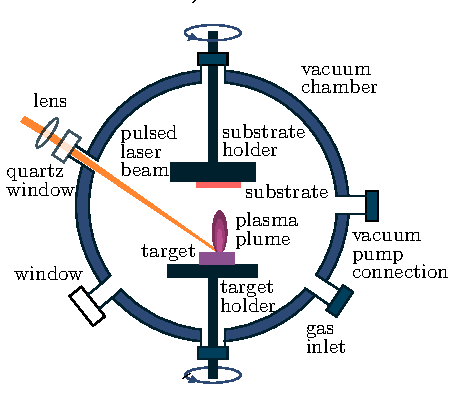
\includegraphics{../assets/pld_chamber}
	\caption{Schematic design of a \ac{pld} chamber.}
	\label{fig:pld_chamber}
\end{figure}
A possible configuration of a \ac{pld} vacuum chamber is shown in 
\cref{fig:pld_chamber}.
The chamber is equipped with a quartz window, used as a laser beam entrance.
Other viewport windows are beneficial for maintenance and monitoring and should
be installed.
These windows should be kept clean to ensure a high transmission of the laser beam
as well as a clear view into the chamber.

There is a vacuum pump connection and gas inlets to regulate a defined
vacuum or atmosphere.
Inside the chamber there are target and substrate holder, that can be rotated and
translated. 
The substrate holder offers various substrate clamps for different substrate sizes.
Usually, a resistive or laser heating system is installed near the substrate holder to
manipulate the substrates temperature and thus the quality of the deposited thin film.
To achieve a more even temperature distribution, the substrate holder is able to rotate.

Towards the substrate holder, a target holder is installed.
This holder is able to rotate and translate as well.
Advanced systems have a target carousel, that can hold multiple targets and can be
rotated to select the desired one.

\subsection{Detailed Working Principle Analysis}
After the \ac{pld} system design has been discussed, the working principle of the
\ac{pld} process shall be explained in detail.
The process can be divided into three main steps: the formation of the laser plasma,
the composition and expansion of the plasma and the nucleation and growth of the film.

\subsubsection{Ablation Process}
Using an adjustable lens, the laser beam is focused onto the target 
with a power density of \qty{10e8}{\watt\per\centi\meter\squared}.
This density is far above the materials thermal evaporation threshold, which is usually 
in order of \qty{10e7}{\watt\per\centi\meter\squared}.
As a result, the target material is ablated and vaporized.
This ablation process is complex and nonequilibrium due to the discontinuous nature 
of the laser pulses.

Thermal ablation by absorption of the laser photons is the most common ablation 
mechanism:
The laser photons are absorbed by the target material.
Due to the high energy of the laser photons, the target material ionizes and 
free electrons are generated.
These free electrons oscillate and can collide with the atoms of the bulk material,
thus transferring energy to the lattice of the target material.
Electromagnetic energy is converted into thermal and chemical energy.
The material is heated up and begins to vaporize.

Apart from thermal ablation, nonthermal, photoinduced electronic sputtering can occur.
This mechanism is based on the direct interaction of the laser photons with the 
electronic system.
Due to electron excitation, chemical bonds can be broken and the material is ejected
from the target, without any significant change in temperature.

Droplets and flakes can be expelled from the target towards the substrate as a result
of plasma recoil pressure and thermal shocks. 
This leads to a reduction of thin film quality.

The target surface is altered during the ablation process, which results in target 
erosion.
This leads to a deviation of the surface normal, therefore changing the plasma 
plume direction.
In order to ensure a uniform material removal, the target is rotated and translated.

\subsubsection{Plasma formation and expansion}
After the material is vaporized, it starts interacting with the laser photons too.
As a result, the material is excited and ionized and a plasma plume is formed.
Due to Coulomb interaction and recoil from the target surface, 
the plasma expands perpendicular to the target surface.

The spatial dependence of the plume depends strongly on the background gas pressure.
At a low background pressures around \qty{10e-4}{\milli \bar} or lower, the plume is
narrow and its constituents have a high velocity.
Only a few scattering events occur.

At intermediate pressures, between \qtyrange{10e-3}{10e-2}{\milli \bar}
a splitting of high energetic ions from less energetic species can be observed.
In high-pressure regions with a background pressure of \qty{10e-1}{\milli \bar} or 
higher, the expansion of the plasma is diffusion-like.
At higher pressures, the plasma plume is wider and the velocity of the species is
reduced.
To underline the influence of the background pressure, the maximum kinetic 
energy of ions with a background pressure of \qty{10e-2}{\milli \bar} is around
\qty{30}{\kilo \electronvolt}, while at \qty{10e-1}{\milli \bar} it is only
\qty{4}{\kilo \electronvolt}.
\begin{figure}
	\centering
	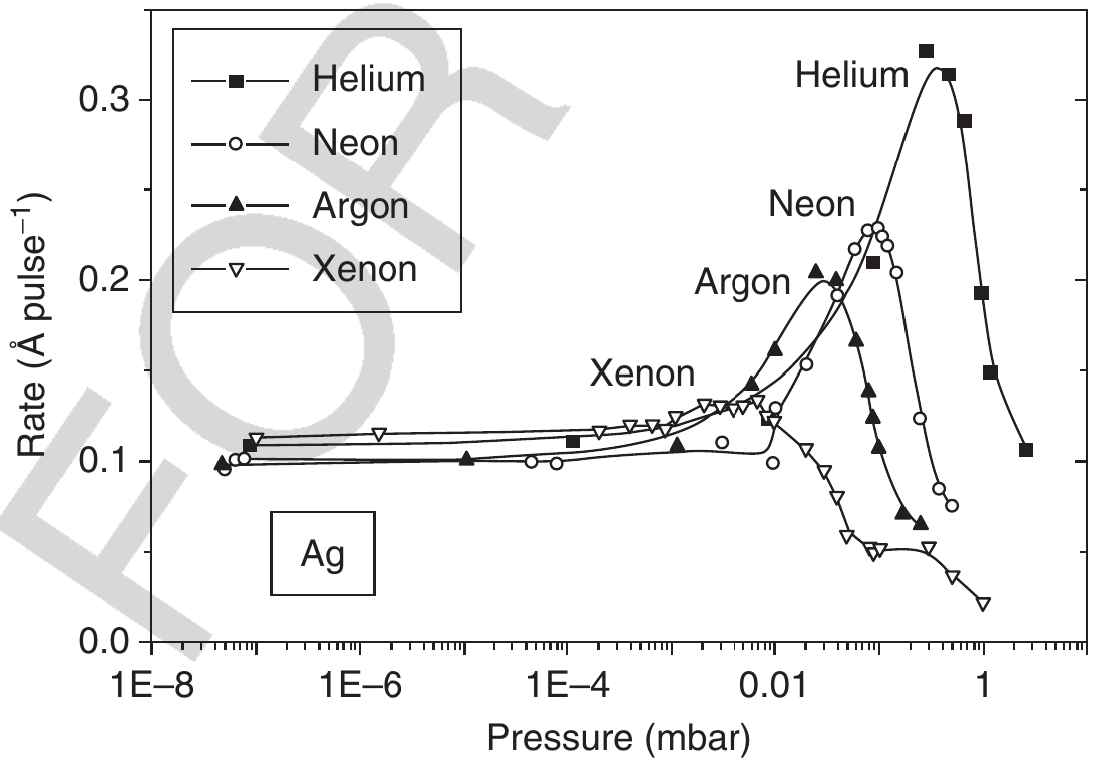
\includegraphics[width=0.98\columnwidth]{../assets/deposition_rate.png}
	\caption{Deposition rate as a function of background pressure for helium, neon, 
	argon and xenon background gases.}
	\label{fig:pld_plasma}
\end{figure}
Not only the kinetic energy of the species is influenced by the background pressure,
but also the deposition rate. 
In \cref{fig:pld_plasma} the deposition rate is shown as a function of the background
pressure for different background gases.
It can be seen that the deposition rate for low background pressures is low.
This is due to the high constituents velocity, which leads to resputtering of the
deposited material.
At higher background pressures, the particle velocity is reduced and the deposition
rate increases.
For even higher pressures, the deposition rate decreases again, 
as a result of the slower and wider spread plasma plume.
Background gas pressure can also lead to a change in stoichiometry of the deposited 
film.
Especially the oxygen concentration in oxide films is strongly influenced by the
background pressure.

\subsubsection{Condensation and Growth of the Film}
The plasma plume is directed towards the substrate, where it condenses on 
the substrate surface and transforms again in a solid state.
A nucleation process starts resulting in thin film growth. 
This step is the most essential for thin film crystal quality.

High-energetic species from the plasma plume are bombarding the substrate
and eventually bond themselves as adatoms. 
This can damage the substrates crystal structure.
Together with other species from the plasma plume, a near-surface collision region is
formed, that serves as a condensation nucleus. 
A large supersaturation occurs on the substrate during the pulse, which leads to a
large nucleation density on the substrate surface.
As a result, other species from the plasma plume append on the condensation nuclei and
the thin film starts to grow.

The growth of the thin film can be divided into three different modes:

\textbf{Layer-by-Layer Growth} is a common growth mode, where monoatomic islands 
emerge until a critical density is reached. 
More ablated material increases the size of the islands until they run into each other.
This is known as coalescence. 
Once coalescence is reached, additional material is used to diffuse into the pits and
complete the first monolayer.
About \numrange{5}{30} laser pulses are required to grow a monolayer.
%TODO add RHEED reference and AC
If the crystal grows layer-by-layer, in situ RHEED delivers very precise control to
measure the number of atomic layers. 

\textbf{3D-Growth} is another growth method, where monoatomic islands 
emerge. 
Once these islands are formed, additional islands nucleate on top.
This leads to three-dimensional islands, which can have different in plane orientations.  

\textbf{Step-Flow Growth} occurs on single-crystalline substrate with a miscut between
the mechanical surface and the crystal lattice planes.
This miscut leads to atomic steps on the surface.
Plasma plume atoms land on the surface and diffuse into a step edge.
This looks like steps travelling across the surface.

The nucleation process depends on various \ac{pld} parameters, including.

\textbf{Laser Parameters}, i.e. laser fluence and laser pulse energy.
Both parameters influence the degree of ionization of the ablated material and therefore
affect deposition flux, thin film quality and stoichiometry. 

\textbf{Substrate Temperature} is another important parameter. 
The nucleation density decreases with increasing substrate temperature, leading to 
fever crystal defects.

\textbf{Substrate Surface} characteristics, i.e. roughness, chemical composition, 
crystal structure and miscut are also a crucial parameter.
Due to the fact that the substrate is the growth template for the thin film, 
the substrate surface determines thin film growth orientation as well as strain and 
defects.

\textbf{Background Pressure} is another important parameter as it determines
the deposition rate as well as the stoichiometry of the deposited film.
It strongly impacts the oxygen proportion in oxide thin films.
High vacuum can lead to oxygen deficiency in the deposited film.

\subsection{PLD in Comparison to other Thin Film Deposition Techniques}
\subsubsection{Sputtering}
\subsubsection{Thermal Evaporation}
\subsubsection{MBE}

\subsubsection{Drawbacks compared to other Techniques}
One big disadvantage of \ac{pld} is the trace element contamination of thin films due
to the spatial expansion of the plasma plume as well as using multiple targets in
one chamber.
Target constituents are located all within the chamber and can lead to permanent damage 
to the windows.
This is a crucial issue, especially for high-purity requirements.
Thin films fabricated by \ac{pld} generally have a higher trace element contamination 
than thin films fabricated by MBE techniques.

It also suffers from target preparation contamination, as the target is prepared by
mechanical ball mills, press molds and sintering ovens.
Also source powders are only available with low purities, which leads to additional 
contamination. 
Traces of construction alloy constituents are also visible at the edge positions of the
thin film. 

Another important disadvantage is the droplet formation during the deposition process.
These droplets can be found in the deposited film and have a size of typically
\qty{1}{\micro \meter}.
This reduces the thin film quality. 
To avoid droplet formation, velocity filters can be used.
Another method would be to arrange the target and the substrate perpendicular to each 
other, such that only the light plasma constituents are scattered towards the substrate.
Both methods reduce the deposition rate of the thin film and complicate the process 
as well.

\subsubsection{Advantages compared to other Techniques}
The biggest advantage of a\ac{pld} system is its flexibility. 
It is a versatile technique for a wide range of thin film and multilayer applications
and offers often a stoichiometric transfer of multielement compounds from a single 
target to a substrate.
With that, it is possible to synthesize chemically complex materials. 
Especially oxide films can be easily controlled by background pressure. 
Most targets can be fabricated with simple lab equipment, for example ball mills and 
sintering furnaces, and commercially available powders.

Reliable and user-friendly excimer lasers are already available. 
The laser operates independently of the deposition system, adhering to a separation 
of concerns design principle, which enhances modularity and simplifies system 
integration.

\ac{pld} systems show an industrial upscaling potential. 
High mass deposition on large areas, with capabilities of covering up to an 8-inch 
diameter surface are already possible. 
Excimer lasers, in particular, provide high pulse energy and a larger focus area at 
lower wavelengths, making them ideal for industrial-scale applications.

\ac{pld} also offers a wide parameter space, making it highly adaptable for various 
applications for and offer tremendous optimization options as well as attractive 
start-up costs.
%\section{Hall effect}
\begin{figure*}
	\centering
	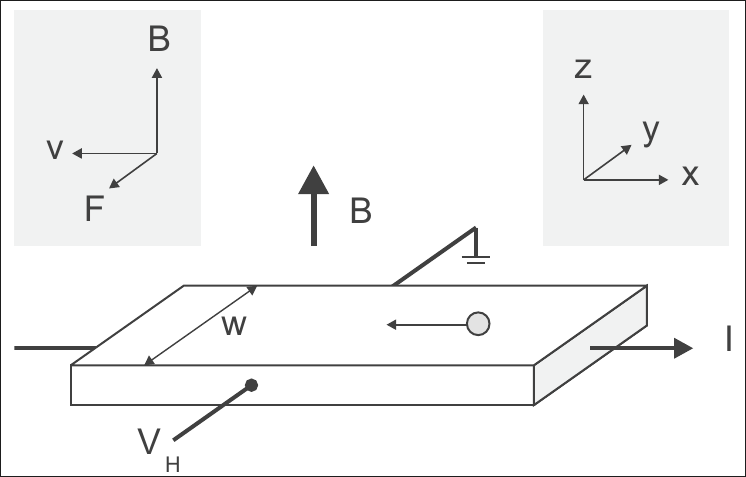
\includegraphics[width=0.8\linewidth]{../assets/hall_geometry.png}
	\caption{Schematic structure for Hall effect measurements.
		\imcite{grundmann}}
	\label{fig:hall}
\end{figure*}
The geometrical arrangement required for Hall effect measurements
is displayed in \cref{fig:hall}.
A magnetic field $\mathbf{B}=B \cdot \hat{z}$ penetrates
a semiconductor sample.
A current $\mathbf{j}$ is flowing along the $x$-direction inside the sample 
as a response to an external electric field $\mathbf{E}=E_x \cdot \hat{x}$.
Due to the magnetic force, the electrons are deflected and a current in
$y$-direction establishes until the resulting electric force in $y$-direction
fully compensates the magnetic force.
The system equilibrates for $j_y=0$.

To describe the system in detail for one majority charge carrier, one can use the 
equation of motion from relaxation time approximation:
\begin{equation}
	m^{*} \frac{\mathbf{v}}{\tau}=q(\mathbf{E}
	+\mathbf{v}\times \mathbf{B}).
\end{equation}
In this equation, $m^{*}$ is the effective mass of the charge carrier, $\mathbf{v}$ the
average electron velocity and $\tau$ the relaxation time constant.
With $\mathbf{j}=nq\mathbf{v}$ and the resistivity tensor $\hat{\rho}$, 
this vector equation can be brought into a linear transformation of the form
$\mathbf{E}=\hat{\rho}\mathbf{j}$ or more explicit:
\begin{equation}
	\label{eq:mej}
	\begin{pmatrix}
		E_{x} \\
		E_{y} \\
		E_{z}
	\end{pmatrix}
	=
	\begin{pmatrix}
		\frac{m^{*}}{\tau nq^{2}} & - \frac{B_{z}}{nq}        & 0                         \\
		\frac{B_{z}}{nq}          & \frac{m^{*}}{\tau nq^{2}} & 0                         \\
		0                         & 0                         & \frac{m^{*}}{\tau nq^{2}}
	\end{pmatrix}
	\begin{pmatrix}
		j_{x} \\
		j_{y} \\
		j_{z}
	\end{pmatrix}.
\end{equation}
The system equilibrates for $\mathbf{j} = j_x \cdot \hat{x}$ and with \cref{eq:mej}, the following
relationship holds true: $E_{y} = B_{z} / (nq) j_{x} = R_{\mathrm{H}}B_{z}j_{x}$.
This leads to an expression for the carrier density $n$ using directly measurable quantities.
\begin{align}
	R_{\mathrm{H}}&=\frac{1}{nq}=\frac{E_{y}}{j_{x}B_{z}}\\
	n&=\frac{j_{x}B_{z}}{E_{y}q}
\end{align}

Now we want to find an expression for the mobility.
\begin{equation}
	\begin{pmatrix}
		E_{x} \\
		E_{y} \\
		E_{z}
	\end{pmatrix}
	=\begin{pmatrix}
		\mu_\mathrm{H}^{-1} & -B_{z}              & 0                   \\
		B_{z}               & \mu_\mathrm{H}^{-1} & 0                   \\
		0                   & 0                   & \mu_\mathrm{H}^{-1}
	\end{pmatrix}
	\begin{pmatrix}
		v_{x} \\
		v_{y} \\
		v_{z}
	\end{pmatrix}
\end{equation}
The hall mobility in this equation is defined as $\mu_{\mathrm{H}}=\frac{q\tau}{m^{*}}$.
To see why this is useful, first, think of the limit $B_{z}\to 0$.
Then, electric field and velocity indeed follow the relation $\mathbf{v}=\mu_{\mathrm{h}}\mathbf{E}$.
Second with $\mathbf{v}=\mu_{\mathrm{h}}\mathbf{E}$ one can easily see that
$v_{x} = \mu_{\mathrm{H}}E_{x}$ and $E_{y}=B_{z}v_{x}=B_{z}\mu_{\mathrm{H}}E_{x}$.
Therefore we find the following equation for $\mu_\mathrm{H}$:
\begin{equation}
	\mu_{\mathrm{H}}=\frac{E_{y}}{B_{z}E_{x}}
\end{equation}

\subsection{Van der Pauw Method}
The Van der Pauw Method is a measuremtn technique to measure the resistivity as well as the hall coefficient.
It is possible to measure samples with nearly arbitrary flat shapes and examine it's resistivity $\rho$, 
mobility $\mu_\mathrm{H}$ as well as it's sheet carrier density $n$. 

Only samples that met the subsequent conditions can be measured with the Van der Pauw method:
\begin{itemize}
	\item The contacts are at the circumference of the sample.
	\item The contacts are sufficiently small (compared to the sample size).
	\item The sample is homogeneous and isotropic cocerning doping as well as thickness.
	\item The surface of the sampele is singly connected, i.e., the sample does not have isolated holes.
\end{itemize}
To utilize the Van der Pauw method, four ohmic contacts need to be placed on the sample.
These contacts should be as small as possible and as close as possible to the samples periphery. 
All contacts and all wires should be constructed from the same material. 

After the ohmic contacts are places, the resistivity $\rho$ can be measured.
Each contact is labeled counterclockwise with a number from 1 to 4.
The current $I_{12}$ is then defined as the positive current injected into contact one and extracted from contact two.
The voltage $V_{34}$ is given by the potential difference between contact three and four as $V_{34}=V_4-V_3$. 
With these definitions, the resistivity can be calculated as $R_{12,34}=\frac{V_{34}}{I_{12}}$. 
Van der Pauw's theorem states that the resistivity can be calculated as 
$$
\begin{align}
\rho&=\frac{\pi d}{\ln(2)} \left( \frac{R_{12,34}+R_{23,41}}{2} \right)f
\left( \frac{R_{12,34}}{R_{23,41}} \right) \\
\label{eq:hall_resistivity}\\
\frac{R_{12,34}-R_{23,41}}{R_{12,34}+R_{23,41}}&=f \, \text{arccosh}\left( \frac{\exp(\ln(2 /f))}{2} \right)
\label{eq:hall_resistivity_f}
\end{align}
$$
where $d$ is the thickness of the sample and $f$ is a correction factor that satisfies \cref{eq:hall_resistivity_f}. 
The reciprocal theorem states that the resistances obey the relation $R_{12,34}=R_{34,12}$ and $R_{12,34}=R_{21,43}$.
Therefore, we can measure the resistivity with four different contact configurations to increase measurement accuracy.

Within the Van der Pauw configuration, it is also possible to determine the Hall coefficient $R_{\mathrm{H}}$ if 
one can establish a homogeneous magnetic field $\mathbf{B}=B_{0} \hat{z}$ perpendicular to the samples surface. 
The Hall coefficient can be calculated as
$$
R_{\mathrm{H}}=\frac{d}{IB_{z}} [U_{13}(B_{z}=0)-U_{13}(B_{z}=B_{0})].
\label{eq:hall_coefficient}
$$
The difference in  \cref{eq:hall_coefficient} accounts for the Hall voltage that originates from the earths magnetic field.




%\section{Results and Discussion}
\subsection{Hall Effect Measurements at Room Temperature}
Measurements were performed on p-type silicon (\ce{p-Si}, $d=\qty{500}{\micro\meter}$), 
zinc oxide (\ce{ZnO}, $d=\qty{1}{\micro\meter}$), zinc tin oxide (\ce{ZTO}, 
$d=\qty{1.3}{\micro\meter}$) and copper iodide (\ce{CuI}, $d=\qty{0.339}{\micro\meter}$) 
thin film samples.
Using the Van der Pauw method, the resistivity, Hall carrier concentration and Hall 
coefficients were determined for each sample.

With four distinct sample contact configurations, four measurements were performed 
per sample. 
The resistivity $\rho$ was calculated using \cref{eq:hall_resistivity}, 
the Hall coefficient $R_{\mathrm{H}}$ using \cref{eq:hall_coefficient_van_der_pauw},
the carrier concentration $n$ using \cref{eq:hall_concentration} 
and the Hall mobility $\mu_{\mathrm{H}}$ using \cref{eq:hall_mobility}.
The results are averaged in \cref{tab:hall_results_detail}, 

An important observation is the varying sign of $R_{\mathrm{H}}$. 
Since the sign of the Hall coefficient is determined by the majority charge carrier
(positive for holes, negative for electrons), this indicates that holes are the majority
charge carrier for \ce{p-Si} and \ce{CuI}. 
Electrons are the majority charge carrier for \ce{ZnO} and \ce{ZTO}. 

\subsection{Temperature Dependent Hall Effect Measurements}
Temperature dependent Hall effect measurements for a bulk \ce{ZnO} sample 
were performed in the Temperature range from \qty{20}{\kelvin} to \qty{325}{\kelvin}.
Both the Hall mobility and Hall carrier concentration were determined for each 
temperature and are displayed in 
\cref{fig:zno_hall_effect_n,fig:zno_hall_effect_mu} respectively.

The graph of the Hall carrier concentration in \cref{fig:zno_hall_effect_n} shows a 
linear decrease with increasing inverse temperature. 
This observation can be explained using the low temperature approximation 
\cref{eq:n_T_approx_low}:

\begin{align}
	&n = \text{const.} \cdot T^{3/2} \exp\left( \frac{-E_{\mathrm{D}}^{b}}{2 \mathrm{k}T} \right) \\
	\ln(&n T^{-3/2}) = \ln(\text{const.}) - \frac{E_{\mathrm{D}}^{b}}{2 \mathrm{k}} \cdot \frac{1}{T} 
	\label{eq:n_T_approx_low_linear}
\end{align}

Using a linear fit, one obtains a slope of \qty{\taskTwoSlope}{\kelvin}.
With \cref{eq:n_T_approx_low_linear}, this slope can be used to determine the donor energy 
$E_{\mathrm{D}}^{b} = \qty{\taskTwoEnergy}{\milli \electronvolt}$.
For high temperatures, the carrier concentration saturates, since all donors are ionized.
By applying \cref{eq:n_T_approx_high}, the donor concentration can be estimated to be
$N_{\mathrm{D}} = \qty{\taskTwoND}{\per \meter\cubed}$.

The Hall mobility in \cref{fig:zno_hall_effect_mu} can be parted into three distinct 
regions.
For every region, the data follows a linear trend, that can be described using three 
linear fits.
The first region has a slope of \num{\taskTwoSlopeOne}, the second region has a slope of
\num{\taskTwoSlopeTwo} 
and the third region has a slope of \num{\taskTwoSlopeThree}.

In a $\log-\log$ plot, a linear function indicates a power law relationship, whereby the
slope of the line corresponds to the exponent of the power law. 
Since the mobility is determined by scattering processes, that have a characteristic 
temperature dependence, different scattering mechanisms can be identified. 
The first region, where $\mu_\mathrm{H} \propto T^{3 / 2}$, can be explained by 
ionized impurity scattering.
The second region, where $\mu_\mathrm{H} \propto T^{\taskTwoSlopeTwo} \simeq T^{-1/2}$, 
can be explained by piezoelectric potential scattering.
The third region, where $\mu_\mathrm{H} \propto T^{\taskTwoSlopeThree} 
\simeq T^{-3 / 2}$, can be explained by deformation potential scattering.

\begin{figure*}
	\centering
	\begin{subfigure}{0.48\textwidth}
		\centering
		\includegraphics{../plots/task_2_n.pdf}
		\caption{Hall carrier concentration of a bulk \ce{ZnO} sample as a function of temperature.}
		\label{fig:zno_hall_effect_n}
	\end{subfigure}
	\hfill
	\begin{subfigure}{0.48\textwidth}
		\centering
		\includegraphics{../plots/task_2_mu.pdf}
		\caption{Hall mobility of a bulk \ce{ZnO} sample as a function of temperature.}
		\label{fig:zno_hall_effect_mu}
	\end{subfigure}
	\caption{Temperature-dependent Hall effect measurements of a bulk \ce{ZnO} sample.}
	\label{fig:zno_hall_effect_combined}
\end{figure*}

\subsection{Interpretation of an Unusual Data Set}
Temperature dependent Hall effect measurements of a \ce{ZnO} thin film sample
were performed in the temperature range from \qty{20}{\kelvin} to \qty{325}{\kelvin}.
However, the dataset does not seem to match a single donor model, as the carrier 
concentration, see \cref{zno_hall_n} raises with falling temperature.
The uncorrected data is shown in \cref{zno_hall_n}, it does not show a linear trend. 

This could indicate that the sample is not a single donor system. 
However, \citeauthoryear{look} suggest, that the sample is a single donor system, 
but a two-layer Hall analysis needs to be performed to correct the data. 
Since \ce{ZnO} and sapphire have a large lattice mismatch, a highly dislocated region 
at the interface between thin film and substrate is generated during growth. 
This high-density region of stacking faults significantly affects the carrier 
concentration as well as the mobility as a function of temperature and does not
show a linear trend.

For a two-layer Hall analysis, we index the \ce{ZnO} thin film as '\num{1}' and the 
dislocated region at the interface as index '\num{2}'. 
Using \cref{eq:multilayer_sum_1,eq:multilayer_sum_2} we can find the following identities
\begin{align}
	\sigma_{\square}=e\mu_{\mathrm{H}1}n_{ \square 1}
	+e \mu_{\mathrm{H}2} n_{ \square 2} \\
	R_{\square} \sigma_{\square}^{2}=e \mu_{\mathrm{H} 1}^{2} n_{ \square 1} 
	+ e\mu_{\mathrm{H} 2}^{2} n_{ \square 2}
\end{align}
It is possible to find an analytical expression for 
$\mu_\mathrm{H}$ and $n$:
\begin{align}
	\mu_{\mathrm{H}}&=R_{\square} \sigma_{\square}
	=\frac{R_{\square} \sigma_{\square}^{2} /d}{\sigma_{\square} / d} \\
	&=\frac{\mu_{\mathrm{H}1}^{2}n_{1}
	+\mu_\mathrm{H2}^{2} n_{\square2} /d}{\mu_{\mathrm{H}1}n_{1}
	+\mu_{\mathrm{H}2}n_{\square{2}} /d} \\
	n_{}=\frac{n_{ \square}}{d}&=\frac{1}{eR_{\square}d}
	= \frac{\sigma^{2}_{\square}/ d^{2}}{eR_{\square}\sigma_{\square}^{2} / d}  \\
	&=\frac{(\mu_{\mathrm{H}1}n_{1}
	+\mu_{\mathrm{H}2}n_{\square2} /d)^{2}}{\mu_{\mathrm{H}1}^{2}n_{1}
	+\mu_{\mathrm{H}2}^{2} n_{ \square 2} /d}
\end{align}
Since the donor atoms freeze at low temperatures, the interface layer must be dominant 
in this region. 
Since the paper suggest that the layer's carrier concentration and mobility is 
temperature independent, we can approximate
$n_{}=n_{ \square 2} / d = \qty{\taskThreeInterfaceN}{\per\meter\cubed}$ 
and 
$\mu_{\mathrm{H}}=\mu_{\mathrm{H 2}} = \qty{\taskThreeInterfaceM}{\centi\meter\squared\per\volt\per\second}$
for $T \to \qty{0}{\kelvin}$. 

An expression for the corrected hall mobility $\mu_{\mathrm{H} 1}$ and  
hall carrier concentration $n_{1}$ can now 
be found:
\begin{align}
	\mu_{\mathrm{H} 1}=\frac{\mu_{\mathrm{H}}^{2} n_{}- \mu_{2} ^{2} 
	n_{ \square 2} /d}{\mu_{\mathrm{H}} n_{} - \mu_{2} n_{\square 2} / d} \\
	n_{1} = \frac{(\mu_{\mathrm{H}}n_{}-\mu_{2}n_{\square 2} 
	/ d)^{2}}{\mu_{\mathrm{H}}^{2}n_{}-\mu_{2}^{2} n_{\square 2} / d}	
\end{align}
The corrected carrier density is also displayed in \cref{zno_hall_n} and can
now be identified with the single-donor case.
Using linear regression, a slope of \num{\taskThreeSlope} and a corresponding donor 
energy of $\qty{\taskThreeEnergy}{\milli \electronvolt}$ can be determined.
The donor concentration can be estimated using \cref{eq:n_T_approx_high} to be
$N_{\mathrm{D}} = \qty{\taskThreeND}{\per\meter \cubed}$

The corrected mobility is displayed in \cref{zno_hall_mu} and shows a linear trend with a 
slope of \num{\taskThreeMobilityOne} for the first region and a slope of 
\num{\taskThreeMobilityThree} for the second region.
The log-log plot indicates a power law relationship, that can be explained by
deformation potential scattering since 
$\mu_\mathrm{H} \propto T^{\taskThreeMobilityThree} \simeq T^{-3/2}$.

\begin{figure*}
	\centering
	\begin{subfigure}[t]{0.48\textwidth}
		\centering
		\includegraphics{../plots/task_3_n.pdf}
		\caption{Corrected and uncorrected Hall carrier concentration of a \ce{ZnO} thin 
		film sample as a function of temperature.}
		\label{zno_hall_n}
	\end{subfigure}
	\hfill
	\begin{subfigure}[t]{0.48\textwidth}
		\centering
		\includegraphics{../plots/task_3_mu.pdf}
		\caption{Corrected and uncorrected Hall mobility of a \ce{ZnO} thin film sample as 
		a function of temperature.}
		\label{zno_hall_mu}
	\end{subfigure}
	\caption{Corrected and uncorrected Hall effect measurements of a \ce{ZnO} thin film sample.}
	\label{fig:zno_hall_effect_corrected}
\end{figure*}

\begin{table*}
\centering
\input{../plots/resistivity_hall.tex}
\caption{Hall effect quantities of p-Si, ZnO, ZTO and CUI thin film samples.}
\label{tab:hall_results_detail}
\end{table*}

\clearpage
\begin{strip}
	\printbibliography[heading=bibintoc]
	\listoffigures
	\listoftables
\end{strip}
$\phantom{=}$
\end{document}
